\documentclass{beamer}

\usepackage{t1enc}
\usepackage[utf8]{inputenc}
\usepackage[magyar]{babel}
\usepackage[useregional]{datetime2}

\usepackage{tikz}
\usetikzlibrary{positioning}
\usetikzlibrary{shapes}
\usetikzlibrary{arrows.meta}
\usepackage{listings}
\usepackage{lstlinebgrd}
\usepackage{pgf, pgffor}
\usepackage{caption}

\input{./misc/highlight.tex}

\lstset{
  language=C,
  basicstyle=\small,
  breaklines=true
  }

\lstset{literate=
 {á}{{\'a}}1 {é}{{\'e}}1 {í}{{\'i}}1 {ó}{{\'o}}1 {ú}{{\'u}}1
 {Á}{{\'A}}1 {É}{{\'E}}1 {Í}{{\'I}}1 {Ó}{{\'O}}1 {Ú}{{\'U}}1
 {ö}{{\"o}}1 {ü}{{\"u}}1 {Ö}{{\"O}}1 {Ü}{{\"U}}1
 {ű}{{\H{u}}}1 {Ű}{{\H{U}}}1 {ő}{{\H{o}}}1 {Ő}{{\H{O}}}1
}

\usetheme{metropolis}
\title{Generátorok előállítása \textit{CPS}-transzformációval Java nyelven}
\date{2017. április 20.}
\author[My name]{Bagossy Attila\\ \footnotesize Témavezetők: Dr. Battyányi Péter, Balla Tibor \vspace{5em}}
\institute{Debreceni Egyetem, Informatikai Kar, Számítógéptudományi Tanszék}

\begin{document}
  \maketitle

  \begin{frame}{Áttekintés}
    \setbeamertemplate{section in toc}[sections numbered]
    \tableofcontents[hideallsubsections]
  \end{frame}

  \section{A generátor és rokonai}


\begin{frame}[fragile]{Szubrutin \textit{(subroutine)}}
Alkalmas kódrészletek kiemelésére, csökkentve a duplikációt.

Meghívása után a hívó kód végrehajtása felfüggesztésre kerül a visszatérésig.
\\
\begin{center}
\begin{minipage}{.40\textwidth}
\begin{lstlisting}[title=Hívó, frame=t, escapechar=!]
!\tikz[remember picture] \node [] (a) {};!/*
  * Kódrészlet
  */
!\tikz[remember picture] \node [] (b) {};! add(2, 2); !\tikz[remember picture] \node [] (c) {};!
 /*
  * Kódrészlet
  */
!\tikz[remember picture] \node [] (f) {};!
\end{lstlisting}
\end{minipage}\hfill
\begin{minipage}{.50\textwidth}
\begin{lstlisting}[title=Szubrutin, frame=t, escapechar=!, showlines=true]
!\tikz[remember picture] \node [] (d) {};! int add(int a, int b)
  {
    /*
     * Kódrészlet
     */
!\tikz[remember picture] \node [] (e) {};! }


\end{lstlisting}
\end{minipage}
\begin{tikzpicture}[remember picture, overlay,
    every edge/.append style = { ->, thick, transparent, >=stealth, line width = 1pt }] 
  \draw (a.north) + (0, 0) coordinate(x1) edge (x1|-b.north);
  \draw (c.east) + (0, 0.15) edge (d.west);
  \draw (d.south) + (0, 0) edge (e.north);
  \draw (e.west) + (0, 0) edge (c.east) + (0, -0.15);
  \draw (b.south) + (0, 0) edge (f.north);
\end{tikzpicture} 
\end{center}
\par
\end{frame}


\begin{frame}[fragile]{Szubrutin \textit{(subroutine)}}
Alkalmas kódrészletek kiemelésére, csökkentve a duplikációt.

Meghívása után a hívó kód végrehajtása felfüggesztésre kerül a visszatérésig.
\\
\begin{center}
\begin{minipage}{.40\textwidth}
\begin{lstlisting}[title=Hívó, frame=t, escapechar=!]
!\tikz[remember picture] \node [] (a) {};!/*
  * Kódrészlet
  */
!\tikz[remember picture] \node [] (b) {};! add(2, 2); !\tikz[remember picture] \node [] (c) {};!
 /*
  * Kódrészlet
  */
!\tikz[remember picture] \node [] (f) {};!
\end{lstlisting}
\end{minipage}\hfill
\begin{minipage}{.50\textwidth}
\begin{lstlisting}[title=Szubrutin, frame=t, escapechar=!, showlines=true]
!\tikz[remember picture] \node [] (d) {};! int add(int a, int b)
  {
    /*
     * Kódrészlet
     */
!\tikz[remember picture] \node [] (e) {};! }


\end{lstlisting}
\end{minipage}
\begin{tikzpicture}[remember picture, overlay,
    every edge/.append style = { ->, thick, >=stealth, line width = 1pt }] 
  \draw (a.north) + (0, 0) coordinate(x1) edge (x1|-b.north);
  \draw (c.east) + (0, 0.15) edge (d.west);
  \draw (d.south) + (0, 0) edge (e.north);
  \draw (e.west) + (0, 0) edge (c.east) + (0, -0.15);
  \draw (b.south) + (0, 0) edge (f.north);
\end{tikzpicture} 
\end{center}
\par
\end{frame}


\begin{frame}[fragile]{Korutin (\textit{coroutine})}
A végrehajtás mindig ott folytatódik, ahol a legutóbbi hívás esetén abbamaradt.

A lokális változók értéke megőrződik a hívások között.
\\
\begin{center}
\begin{minipage}{.40\textwidth}
\begin{lstlisting}[escapechar=!, keywords={coroutine, yield}]
coroutine A()
{
    /* ... */
    yield B; !\tikz[remember picture] \node [] (a) {};!
    /* ... */!\tikz[remember picture] \node [] (d) {};!
    yield B; !\tikz[remember picture] \node [] (e) {};!
}
\end{lstlisting}
\end{minipage}\hfill
\begin{minipage}{.50\textwidth}
\begin{lstlisting}[escapechar=!, showlines=true, keywords={coroutine, yield}]
coroutine B()
{
    !\tikz[remember picture] \node [] (b) {};! /* ... */
    !\tikz[remember picture] \node [] (c) {};! yield A; 
    !\tikz[remember picture] \node [] (f) {};! /* ... */
}

\end{lstlisting}
\end{minipage}
\begin{tikzpicture}[remember picture, overlay,
    every edge/.append style = { ->, thick, transparent, >=stealth, line width = 1pt }] 
  \draw (a.east) + (0, 0) edge (b.west);
  \draw (c.west) + (0, 0) edge (d.east);
  \draw (e.east) + (0, 0) edge (f.west);
\end{tikzpicture} 
\end{center}
\par
\end{frame}


\begin{frame}[fragile]{Korutin (\textit{coroutine})}
A végrehajtás mindig ott folytatódik, ahol a legutóbbi hívás esetén abbamaradt.

A lokális változók értéke megőrződik a hívások között.
\\
\begin{center}
\begin{minipage}{.40\textwidth}
\begin{lstlisting}[escapechar=!, keywords={coroutine, yield}]
coroutine A()
{
    /* ... */
    yield B; !\tikz[remember picture] \node [] (a) {};!
    /* ... */!\tikz[remember picture] \node [] (d) {};!
    yield B; !\tikz[remember picture] \node [] (e) {};!
}
\end{lstlisting}
\end{minipage}\hfill
\begin{minipage}{.50\textwidth}
\begin{lstlisting}[escapechar=!, showlines=true, keywords={coroutine, yield}]
coroutine B()
{
    !\tikz[remember picture] \node [] (b) {};! /* ... */
    !\tikz[remember picture] \node [] (c) {};! yield A; 
    !\tikz[remember picture] \node [] (f) {};! /* ... */
}

\end{lstlisting}
\end{minipage}
\begin{tikzpicture}[remember picture, overlay,
    every edge/.append style = { ->, thick, >=stealth, line width = 1pt }] 
  \draw[orange] (a.east) + (0, 0) edge (b.west);
  \draw[transparent] (c.west) + (0, 0) edge (d.east);
  \draw[transparent] (e.east) + (0, 0) edge (f.west);
\end{tikzpicture} 
\end{center}
\par
\end{frame}


\begin{frame}[fragile]{Korutin (\textit{coroutine})}
A végrehajtás mindig ott folytatódik, ahol a legutóbbi hívás esetén abbamaradt.

A lokális változók értéke megőrződik a hívások között.
\\
\begin{center}
\begin{minipage}{.40\textwidth}
\begin{lstlisting}[escapechar=!, keywords={coroutine, yield}]
coroutine A()
{
    /* ... */
    yield B; !\tikz[remember picture] \node [] (a) {};!
    /* ... */!\tikz[remember picture] \node [] (d) {};!
    yield B; !\tikz[remember picture] \node [] (e) {};!
}
\end{lstlisting}
\end{minipage}\hfill
\begin{minipage}{.50\textwidth}
\begin{lstlisting}[escapechar=!, showlines=true, keywords={coroutine, yield}]
coroutine B()
{
    !\tikz[remember picture] \node [] (b) {};! /* ... */
    !\tikz[remember picture] \node [] (c) {};! yield A; 
    !\tikz[remember picture] \node [] (f) {};! /* ... */
}

\end{lstlisting}
\end{minipage}
\begin{tikzpicture}[remember picture, overlay,
    every edge/.append style = { ->, thick, , >=stealth, line width = 1pt }] 
  \draw (a.east) + (0, 0) edge (b.west);
  \draw[orange] (c.west) + (0, 0) edge (d.east);
  \draw[transparent] (e.east) + (0, 0) edge (f.west);
\end{tikzpicture} 
\end{center}
\par
\end{frame}


\begin{frame}[fragile]{Korutin (\textit{coroutine})}
A végrehajtás mindig ott folytatódik, ahol a legutóbbi hívás esetén abbamaradt.

A lokális változók értéke megőrződik a hívások között.
\\
\begin{center}
\begin{minipage}{.40\textwidth}
\begin{lstlisting}[escapechar=!, keywords={coroutine, yield}]
coroutine A()
{
    /* ... */
    yield B; !\tikz[remember picture] \node [] (a) {};!
    /* ... */!\tikz[remember picture] \node [] (d) {};!
    yield B; !\tikz[remember picture] \node [] (e) {};!
}
\end{lstlisting}
\end{minipage}\hfill
\begin{minipage}{.50\textwidth}
\begin{lstlisting}[escapechar=!, showlines=true, keywords={coroutine, yield}]
coroutine B()
{
    !\tikz[remember picture] \node [] (b) {};! /* ... */
    !\tikz[remember picture] \node [] (c) {};! yield A; 
    !\tikz[remember picture] \node [] (f) {};! /* ... */
}

\end{lstlisting}
\end{minipage}
\begin{tikzpicture}[remember picture, overlay,
    every edge/.append style = { ->, thick, >=stealth, line width = 1pt }] 
  \draw (a.east) + (0, 0) edge (b.west);
  \draw (c.west) + (0, 0) edge (d.east);
  \draw[orange] (e.east) + (0, 0) edge (f.west);
\end{tikzpicture} 
\end{center}
\par
\end{frame}


\begin{frame}[fragile]{Generátor (\textit{generator})}
Aszimmetrikus korutin, amely elemek sorozatát állítja elő.

\hfill \\

Minden egyes hívás alkalmával a sorozat egy elemét képzi.

\begin{center}
\begin{minipage}{.40\textwidth}
\begin{lstlisting}[escapechar=!, showlines=true, keywords={for, in, print}]
for ch in alphabet()
{
    print ch
}



\end{lstlisting}
\end{minipage}\hfill
\begin{minipage}{.50\textwidth}
\begin{lstlisting}[escapechar=!, showlines=true, keywords={generator, yield}]
generator alphabet()
{
    yield 'a';
    yield 'b';
    yield 'c';
    /* ... */
}
\end{lstlisting}
\end{minipage}
\end{center}
\par
\end{frame}

  \section{Generátorok ismert nyelvekben}

\begin{frame}{Támogatást biztosító nyelvek}
    \begin{block}{Első, úttörő próbálkozások}
        \indent\textit{IPL-V}, \textit{Alphard}
    \end{block}
    \begin{block}{A \texttt{yield} kulcsszó bevezetése}
        \textit{CLU}
    \end{block}
    \begin{block}{TIOBE Top 10, 2017. március}
        \begin{itemize}
            \item
            \textit{C\#}
            \item
            \textit{Python}
            \item
            \textit{Visual Basic .NET}
            \item
            \textit{PHP}
            \item
            \textit{JavaScript}
        \end{itemize}
    \end{block}
\end{frame}


\begin{frame}{Felhasználási lehetőségek -- 1}
\begin{block}{Végtelen sorozatok}
    \begin{itemize}
        \item
        Fibonacci sorozat
        \item
        Prímszámok
        \item
        Véletlen értékek forrása
    \end{itemize}
\end{block}
\begin{block}{Véges sorozatok}
    \begin{itemize}
        \item
        Reguláris kifejezésre illesztés eredményei
        \item
        Fájl beolvasása soronként/darabonként
        \item
        Paraméteres görbék pontjai
    \end{itemize}
\end{block}
\end{frame}


\begin{frame}{Felhasználási lehetőségek -- 2}
\begin{itemize}
    \item
    Szimmetrikus korutinok modellezése \\
    \hfill \\
    \item
    \texttt{async/await} szimulálása (\textit{JavaScript}) \\
    \hfill \\
    \item
    Mikroszálak létrehozása, ütemezése
\end{itemize}
\end{frame}


  \section{Korábbi Java implementációk}

\begin{frame}{Általános problémák}
Csak régebbi \textit{Java} verziók támogatása (\textit{Java SE} 6-7)


\hfill \\

\pause
Kényelmetlen interfész


\hfill \\

\pause
Rugalmatlan, kevésbé megbízható megvalósítás
\end{frame}


\begin{frame}[fragile]{jyield}
\begin{center}
\begin{lstlisting}[language=java, xleftmargin=15pt,
        basicstyle=\scriptsize,
        numbers=left,
        numbersep=5pt, escapechar=!]
@Continuable
public Iterable<Integer> power(int number, int exponent) 
{
        int counter = 0;
        int result = 1;
        while (counter++ < exponent) {
                result = result * number;

                System.out.print("[" + result + "]");

                Yield.ret(result);
        }
        return Yield.done();
}
\end{lstlisting}
\end{center}
\par
\end{frame}


\begin{frame}[fragile]{java-generator-functions}
\begin{center}
\begin{lstlisting}[language=java, xleftmargin=15pt,
        basicstyle=\scriptsize,
        numbers=left,
        numbersep=5pt, escapechar=!]
Generator<Integer> simpleGenerator = 
  new Generator<Integer>() {
    public void run() throws InterruptedException {
        yield(1);
        /* ... */
        yield(2);
    }
};
\end{lstlisting}
\end{center}
\par
\end{frame}


\begin{frame}[fragile]{lombok-pg}
\begin{center}
\begin{lstlisting}[language=java, xleftmargin=15pt,
        basicstyle=\scriptsize,
        numbers=left,
        numbersep=5pt, escapechar=!]
public Iterable<Integer>
  power(final int number, final int exponent) 
{
        int counter = 0;
        int result = 1;
        while (counter++ < exponent) {
                result = result * number;

                System.out.print("[" + result + "]");

                yield(result);
        }
}
\end{lstlisting}
\end{center}
\par
\end{frame}

  \section{Az eljárás egy példán keresztül}

\begin{frame}{Az eljárás jellemzői}
A \textit{Pluggable Annotation Processing} API-t használja


\hfill \\

\pause
A \texttt{return} utasítás jelképezi a \texttt{yield} utasítást


\hfill \\

\pause
\textit{Continuation Passing Style}-alapú megvalósítás
\end{frame}


\begin{frame}[fragile]{Prímek generálása}
\begin{center}
\begin{lstlisting}[language=java, xleftmargin=15pt,
        basicstyle=\fontsize{7}{9}\selectfont,
        numbers=left,
        numbersep=5pt, escapechar=!,
        linebackgroundcolor={
            \btLstHL<1>{30} % No highlighting
            \btLstHL<2>{5}
            \btLstHL<3>{20}
        }]
@Generator
private Stream<Integer> generatePrimes() {
    LinkedList<Integer> primes = new LinkedList<>();
    primes.add(2);
    return 2;

    int current = 1;

    loop:
    do {
        current += 2;
        for (int i : primes) {
            if (current % i == 0) {
                continue loop;
            }
        }

        primes.add(current);

        return current;
    } while (true);
}
\end{lstlisting}
\end{center}
\par
\end{frame}


\begin{frame}[fragile]{Prímek generálása -- Vágási pontok}
\begin{center}
\begin{lstlisting}[language=java, xleftmargin=15pt,
        basicstyle=\fontsize{7}{9}\selectfont,
        numbers=left,
        numbersep=5pt, escapechar=!,
        linebackgroundcolor={
            \btLstHL<1>{30} % No highlighting
            \btLstHL<2>{5, 20}
            \btLstHL<3>{10, 21}
            \btLstHL<4>{14}
            \btLstHL<5>{12-16}
        }]
@Generator
private Stream<Integer> generatePrimes() {
    LinkedList<Integer> primes = new LinkedList<>();
    primes.add(2);
    return 2;

    int current = 1;

    loop:
    do {
        current += 2;
        for (int i : primes) {
            if (current % i == 0) {
                continue loop;
            }
        }

        primes.add(current);

        return current;
    } while (true);
}
\end{lstlisting}
\end{center}
\par
\end{frame}


\begin{frame}{A vezérlés útja}
\begin{center}
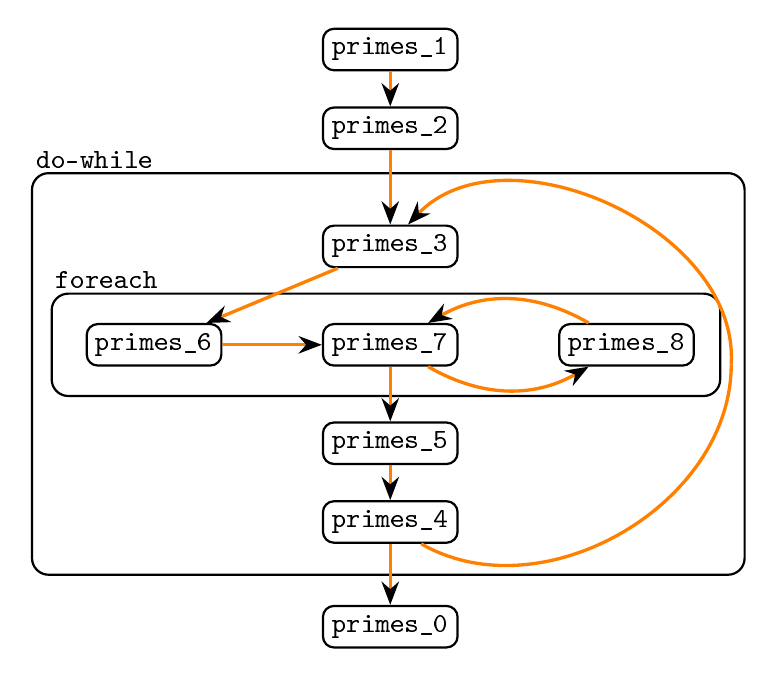
\begin{tikzpicture}
\begin{scope}
    \draw[thick, rounded corners=6pt]  (-4.55, -1.57) rectangle (4.5, -6.67);

    \draw[thick, rounded corners=6pt]  (-4.3, -3.10) rectangle (4.19, -4.4);
\end{scope}

\begin{scope}
  \node at (-3.75, -1.4) {\texttt{do-while}};

  \node at (-3.6, -2.93) {\texttt{foreach}};
\end{scope}

\begin{scope}[every node/.style={thick,draw, rounded corners=4pt}]
  \node (1) at (0, 0) {\texttt{primes\_1}};
  \node (2) at (0, -1) {\texttt{primes\_2}};
  \node (3) at (0, -2.5) {\texttt{primes\_3}};
  \node (5) at (0, -5) {\texttt{primes\_5}};
  \node (4) at (0, -6) {\texttt{primes\_4}};
  \node (6) at (-3, -3.75) {\texttt{primes\_6}};
  \node (7) at (0, -3.75) {\texttt{primes\_7}};
  \node (8) at (3, -3.75) {\texttt{primes\_8}};
  \node (0) at (0, -7.33) {\texttt{primes\_0}};
\end{scope}

\begin{scope}[>={Stealth[black]},
              every edge/.style={draw=orange, very thick}]
    \path [->] (1) edge (2);
    \path [->] (2) edge (3);
    \path [->] (3) edge (6);
    \path [->] (6) edge (7);
    \path [->] (7) edge[bend right=30] (8);
    \path [->] (8) edge[bend right=30] (7);
    \path [->] (7) edge (5);
    \path [->] (5) edge (4);
    \path [->] (4) edge (0);
    \path (4) edge[bend right=60]  (4.33, -4);
    \path[->] (4.33, -4) edge[bend right=70] (3);
\end{scope}
\end{tikzpicture}
\end{center}
\end{frame}


\lstset{language=java, xleftmargin=15pt,
        basicstyle=\scriptsize,
        numbers=left,
        numbersep=5pt, escapechar=!}

\begin{frame}[fragile]{A transzformáció lépései -- 1}
\begin{lstlisting}
private Bounce<Integer> primes_0(GenState<Integer> k) {
    return Bounce.cont(()->k.apply(GenState.empty()));
}
\end{lstlisting}
\end{frame}


\begin{frame}[fragile]{A transzformáció lépései -- 2}
\begin{center}\textbf{Eredeti kód}\end{center}
\begin{lstlisting}[linebackgroundcolor={
            \btLstHL<1>{30} % No highlighting
            \btLstHL<2>{1}
            \btLstHL<3>{3}
        }]
 LinkedList<Integer> primes = new LinkedList<>();
 primes.add(2);
 return 2;
\end{lstlisting}

\begin{center}\textbf{Transzformált kód}\end{center}
\begin{lstlisting}[linebackgroundcolor={
            \btLstHL<1>{30} % No highlighting
            \btLstHL<2>{2}
            \btLstHL<3>{4}
        }]
 private Bounce<Integer> primes_1(GenState<Integer> k) {
     primes = new LinkedList<>();
     primes.add(2);
     return Bounce.cont(()->primes_2(k), 2);
 }
\end{lstlisting}
\end{frame}


\begin{frame}[fragile]{A transzformáció lépései -- 3}
\begin{center}\textbf{Eredeti kód}\end{center}
\begin{lstlisting}[linebackgroundcolor={
            \btLstHL<1>{30} % No highlighting
            \btLstHL<2>{6}
            \btLstHL<3>{30} % No highlighting
            \btLstHL<4>{30} % No highlighting
        }]
 loop:
 do {
     /*
      * Törzs
      */
 } while (true);
\end{lstlisting}

\begin{center}\textbf{Transzformált kód}\end{center}
\begin{lstlisting}[linebackgroundcolor={
            \btLstHL<1>{30} % No highlighting
            \btLstHL<2>{2}
            \btLstHL<3>{3}
            \btLstHL<4>{5}
        }]
 private Bounce<Integer> primes_4(GenState<Integer> k) {
     if (true) {
         return Bounce.cont(()->primes_3(k));
     }
     return Bounce.cont(()->primes_0(k));
 }
\end{lstlisting}
\end{frame}


\begin{frame}[fragile]{A transzformáció lépései -- 4}
\begin{center}\textbf{Eredeti kód}\end{center}
\begin{lstlisting}[linebackgroundcolor={
            \btLstHL<1>{1}
        }]
 current += 2;
 for (int i : primes) {
     if (current % i == 0) {
         continue loop;
     }
 }
 
 primes.add(current);
 
 return current;
\end{lstlisting}

\begin{center}\textbf{Transzformált kód}\end{center}
\begin{lstlisting}
 private Bounce<Integer> primes_3(GenState<Integer> k) {
     current += 2;
     return Bounce.cont(()->primes_6(k));
 }
\end{lstlisting}
\end{frame}

\begin{frame}[fragile]{A transzformáció lépései -- 4}
\begin{center}\textbf{Eredeti kód}\end{center}
\begin{lstlisting}[linebackgroundcolor={
            \btLstHL<1>{8-10}
        }]
 current += 2;
 for (int i : primes) {
     if (current % i == 0) {
         continue loop;
     }
 }
 
 primes.add(current);
 
 return current;
\end{lstlisting}

\begin{center}\textbf{Transzformált kód}\end{center}
\begin{lstlisting}
 private Bounce<Integer> primes_5(GenState<Integer> k) {
     primes.add(current);
     return Bounce.cont(()->primes_4(k), current);
 }
\end{lstlisting}
\addtocounter{framenumber}{-1}
\end{frame}



\begin{frame}[fragile]{A transzformáció lépései -- 5}
\begin{center}\textbf{Eredeti kód}\end{center}
\begin{lstlisting}[linebackgroundcolor={
            \btLstHL<1>{1}
        }]
 for (int i : primes) {
     if (current % i == 0) {
         continue loop;
     }
 }
\end{lstlisting}

\begin{center}\textbf{Transzformált kód}\end{center}
\begin{lstlisting}
 private Bounce<Integer> primes_6(GeState<Integer> k) {
     iterator = CPSUtil.iterator(primes);
     return Bounce.cont(()->primes_7(k));
 }
\end{lstlisting}
\end{frame}


\begin{frame}[fragile]{A transzformáció lépései -- 5}
\begin{center}\textbf{Eredeti kód}\end{center}
\begin{lstlisting}[linebackgroundcolor={
            \btLstHL<1>{1}
        }]
 for (int i : primes) {
     if (current % i == 0) {
         continue loop;
     }
 }
\end{lstlisting}

\begin{center}\textbf{Transzformált kód}\end{center}
\begin{lstlisting}
 private Bounce<Integer> primes_7(GenState<Integer> k) {
     if (iterator.hasNext()) {
         i = iterator.next();
         return Bounce.cont(()->primes_8(k));
     }
     return Bounce.cont(()->primes_5(k));
 }
\end{lstlisting}
\addtocounter{framenumber}{-1}
\end{frame}


\begin{frame}[fragile]{A transzformáció lépései -- 5}
\begin{center}\textbf{Eredeti kód}\end{center}
\begin{lstlisting}[linebackgroundcolor={
            \btLstHL<1>{2-4}
        }]
 for (int i : primes) {
     if (current % i == 0) {
         continue loop;
     }
 }
\end{lstlisting}

\begin{center}\textbf{Transzformált kód}\end{center}
\begin{lstlisting}
 private Bounce<Integer> primes_8(GenState<Integer> k) {
     if (current % i == 0) {
         return Bounce.cont(()->primes_4(k));
     }
     return Bounce.cont(()->primes_7(k));
 }
\end{lstlisting}
\addtocounter{framenumber}{-1}
\end{frame}        


\begin{frame}{A vezérlés útja}
\begin{center}
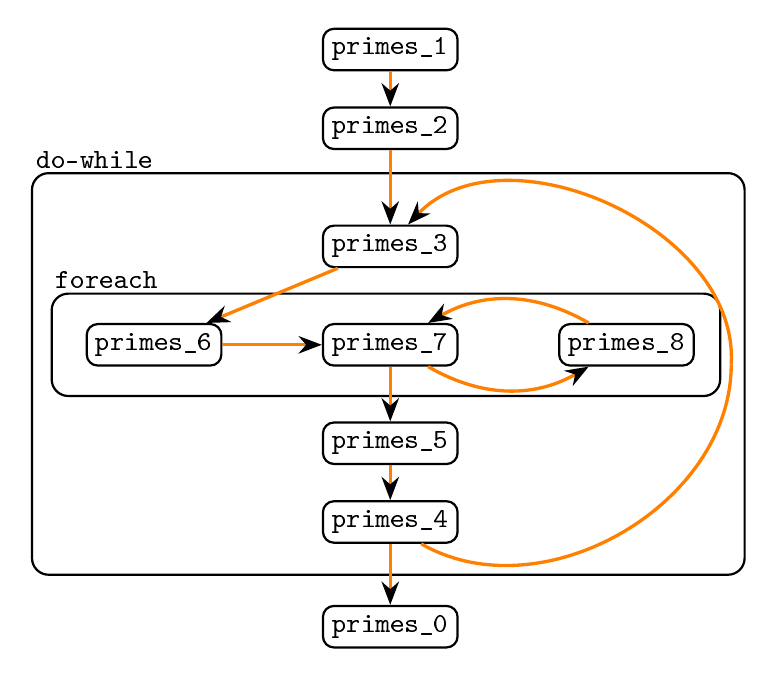
\begin{tikzpicture}
\begin{scope}
    \draw[thick, rounded corners=6pt]  (-4.55, -1.57) rectangle (4.5, -6.67);

    \draw[thick, rounded corners=6pt]  (-4.3, -3.10) rectangle (4.19, -4.4);
\end{scope}

\begin{scope}
  \node at (-3.75, -1.4) {\texttt{do-while}};

  \node at (-3.6, -2.93) {\texttt{foreach}};
\end{scope}

\begin{scope}[every node/.style={thick,draw, rounded corners=4pt}]
  \node (1) at (0, 0) {\texttt{primes\_1}};
  \node (2) at (0, -1) {\texttt{primes\_2}};
  \node (3) at (0, -2.5) {\texttt{primes\_3}};
  \node (5) at (0, -5) {\texttt{primes\_5}};
  \node (4) at (0, -6) {\texttt{primes\_4}};
  \node (6) at (-3, -3.75) {\texttt{primes\_6}};
  \node (7) at (0, -3.75) {\texttt{primes\_7}};
  \node (8) at (3, -3.75) {\texttt{primes\_8}};
  \node (0) at (0, -7.33) {\texttt{primes\_0}};
\end{scope}

\begin{scope}[>={Stealth[black]},
              every edge/.style={draw=orange, very thick}]
    \path [->] (1) edge (2);
    \path [->] (2) edge (3);
    \path [->] (3) edge (6);
    \path [->] (6) edge (7);
    \path [->] (7) edge[bend right=30] (8);
    \path [->] (8) edge[bend right=30] (7);
    \path [->] (7) edge (5);
    \path [->] (5) edge (4);
    \path [->] (4) edge (0);
    \path (4) edge[bend right=60]  (4.33, -4);
    \path[->] (4.33, -4) edge[bend right=70] (3);
\end{scope}
\end{tikzpicture}
\end{center}
\end{frame}


  \begin{frame}{Összefoglalás}
    A generátorok bevezetése \textit{Java}ban indokolt, hiszen rendkívül rugalmasan felhasználhatóak.

    \hfill \\

    A bemutatott eljárás mindössze egy annotáció elhelyezését igényli a programozó részéről.

    \hfill \\

    A háttérben a metódusok kisebb darabokra vágása történik meg, melyeket futásidőben egy \textit{trampoline} vezérel.

    \hfill \\

    A vezérlési szerkezeteket elágazások és megfelelő módon szervezett \textit{continuation}ök modellezik.
  \end{frame}

  \begin{frame}[standout]
    Köszönöm a figyelmet!
  \end{frame}

  % \section{Continuation Passing Style}

\begin{frame}{Mi a \textit{continuation}?}
A hátralevő számításokat reprezentálja, hogy \textit{mi a következő teendő}.

\hfill \\

Absztrakt fogalom, mely többféle módon is realizálható.

\hfill \\

Leggyakrabban egy függvény jelenti a \textit{continuation}t.
\end{frame}

\begin{frame}{\textit{CPS} szabályok}
\begin{enumerate}
\item
A függvények sohasem térhetnek vissza.
\item
Minden függvény paraméterlistája kiegészül egy (vagy több) \textit{continuation}t jelképező paraméterrel.
\end{enumerate}
\end{frame}
\end{document}
